The PID controller (P-proportional,  I-integral, D-derivative) controller is the most widely used process control. Its control signal uses three actions on a manipulated variable to reach a specific set point.\\

\textbf{Proportional} action emits a signal proportional to the control error (control error = desired value - output value of the process).\newline
\textbf{Integral} action ensures that the steady state error is zero process, ie the process value output is equal to the desired value.\newline
The \textbf{derivative} action improves the stability of the control loop, it predicts the error value Td time forward.\\

\begin{figure}[H]
\centering
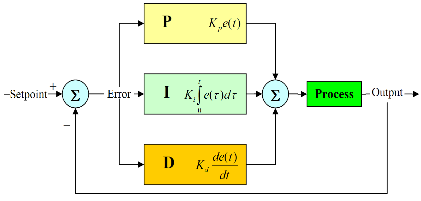
\includegraphics{images/pid}
\caption{Block diagram for a general PID controller}
\label{fig:pid}
\end{figure}

\clearpage

The PID control algorithm tries to stabilze the system about its mean position. The mean poition in the case of the self balancing bot is the pitch position at which it experiences zero torque from its own weight. The mean position in case of the self-balancing table is the position at which it is perfectly level with respect to the ground. The control algorithm is used to maintain the bot and the table individually at this mean position individually.
The response is made desirable by setting the PID values by following the steps given in the following chapter on 'Tuning'. \\

The system attempts to minimize the error by adjusting the process by relying only on the measured process variable, not on knowledge of the underlying process. Therefore, it requires minimal modelling and doesn't require excessive mathematical manipulations, making it simple to implement in low-power embedded systems.
